\def\year{2016}\relax
%File: formatting-instruction.tex
\documentclass[letterpaper]{article}
\usepackage{aaai16}
\usepackage{times}
\usepackage{helvet}
\usepackage{courier}
\usepackage{graphicx}
\usepackage{amsfonts}
\frenchspacing
\setlength{\pdfpagewidth}{8.5in}
\setlength{\pdfpageheight}{11in}
\pdfinfo{
/Title (Insert Your Title Here)
/Author (Put All Your Authors Here, Separated by Commas)}
\setcounter{secnumdepth}{0}  
 \begin{document}
% The file aaai.sty is the style file for AAAI Press 
% proceedings, working notes, and technical reports.
%
%\title{Formatting Instructions \\for Authors Using \LaTeX{}}
\title{Attention-based Sequence to Sequence Model for Tweet Normalization}
\author{AAAI Press\\
Association for the Advancement of Artificial Intelligence\\
2275 East Bayshore Road, Suite 160\\
Palo Alto, California 94303\\
}
\maketitle
\begin{abstract}
	Paraphrase identification for tweet is a new challenge due to informal expression. In this paper, we present a end-to-end approach to sequence learning that transfers text normalization into a neural machine translation task. Then a siamese recurrent architecture is used for learning sentence similarity after the sentences have been normalized. Our model employs a convolutional neural network and a highway network over characters, whose output is given to a long short-term memory recurrent neural network to map the input sequence to a vector of a fixed dimensionality, and then another long short-term memory to decode the target sequence from the vector. We add an attentional mechanism to improve the performance of tweet normalization, which can be beneficial to paraphrase detection indirectly. Novelty of this work is three-fold: First, to the best of our knowledge, this is an early attempt to adopt attention-based end-to-end model for tweet normalization. Second, our proposed model relies on	character-level inputs, making it fewer parameters to obtain comparable performance to word inputs. And third, we conduct a series of experiments and prove that the proposed method is advantageous over the state-of-art solutions for tweet normalization and semantic similarity. Our method shows significant performance gains on the paraphrase identification in tweet task compared with several strong baselines. 
\end{abstract}

\section{Introduction}
Semantic similarity of text are used in many semantic tasks such as paraphrase identification \cite{Xu-EtAl-2014:TACL}, textual entailment \cite{henderson-popa:2016:P16-1}, and question answering \cite{Severyn:2015:LRS:2766462.2767738}. Twitter engages millions of users, who naturally talk about the same topics simultaneously and frequently convey similar meaning using diverse linguistic expressions. The unique characteristics of this user-generated text presents new challenges and opportunities for semantic similarity measurement. Unfortunately, traditional natural language processing methods sometimes perform poorly when processing this kind of text. One reason is that tweets are very informal, and contain many misspelled words, abbreviations and many other non-standard tokens, which make it substantially different from formal written text. To improve the performance on the social media semantic similarity, it is inevitable to leverage normalization techniques which can automatically convert the non-standard tokens into the corresponding standard words.

Intuitively, tweet normalization will be beneficial for paraphrase identification and textual  semantic similarity. For example, if `tmr' is converted to `tomorrow', it will improve the semantic representation for tweets and promote similarity comparison performance between text pairs. This normalization task has received an increasing in social media language processing. However, most of previous work on normalization assumed that they already knew which tokens are non-standard words (NSW) that need normalization. Then different methods are applied only to these tokens. Han and Baldwin \shortcite{han-baldwin:2011:ACL-HLT2011} is the typical work which made a pilot reasearch on NSW identification. One straight forward method to do this is to use a dictionary to classify a token into in-vocabulary (IV) words and out-of-vocabulary (OOV) words, and just treat all the OOV words as NSW. Contrast to straight forward work, joint part-of-speech (POS) and text normalization was proposed by Li and Liu \shortcite{Li:2015:JPT:2832415.2832425}, the objective of this work is to perform POS tagging and text normalization at the same time. It indicates the thought that joint tweet normalization and similarity.

Character-aware neural language model \cite{Kim-AAAI1612489} relies only on character-level inputs and predictions are still made at the word-level, and the model can leverage subword information through a character-level convolutional neural network (CNN) and have a good performance on the estimation of rare words embeddings. Therefore, it is attracting to explore neual language model for tweet normalization. Xu et al. \shortcite{xu-callisonburch-dolan:2015:SemEval} proposed a share task evaluation on both  paraphrase identification and semantic textual similarity for Twitter data. Although some works \cite{zarrella-EtAl:2015:SemEval,vandergoot-vannoord:2015:SemEval} take tweet normalization into account, this researches are limited to replace the OOV words with normalization dictionary.

In this paper, we proposed a character-level neural language model for tweet normalization, and then measure the semantic of normalized text for paraphrase identification and textual similarity. Our work investigates two methods using normalized tweets for sematic similarity measurement. One adopts a pipline strategy, and the other uses a joint fashion. Our experimental results demonstrate that our proposed model gives a significant performance improvement on NSW detection compared with the dictionary baseline system and our proposed joint model performs better than the pipeline method, and it outperforms the state-of-the-art paraphrase identification system. To summarize, our contributions in this paper are as follows:

\begin{itemize}
	\item We proposed a character-level neural language model for tweet normalization, which achieve results on par with the existing state-of-the-art NSW detection.
	\item The proposed joint model can combine the normalization and semantic textual similarity techniques to improve the fprmance of these two tasks on English social media data.
	\item We demonstrate the effectiveness of our proposed method. Experimental results achieve the state-of-the-art performance on normalization and similarity.
\end{itemize}

\section{Model}
The proposed model adopt a sequence to sequence method for learning a neural language model. We illustrate these two model types in Figure 1.
\begin{figure}
\centering
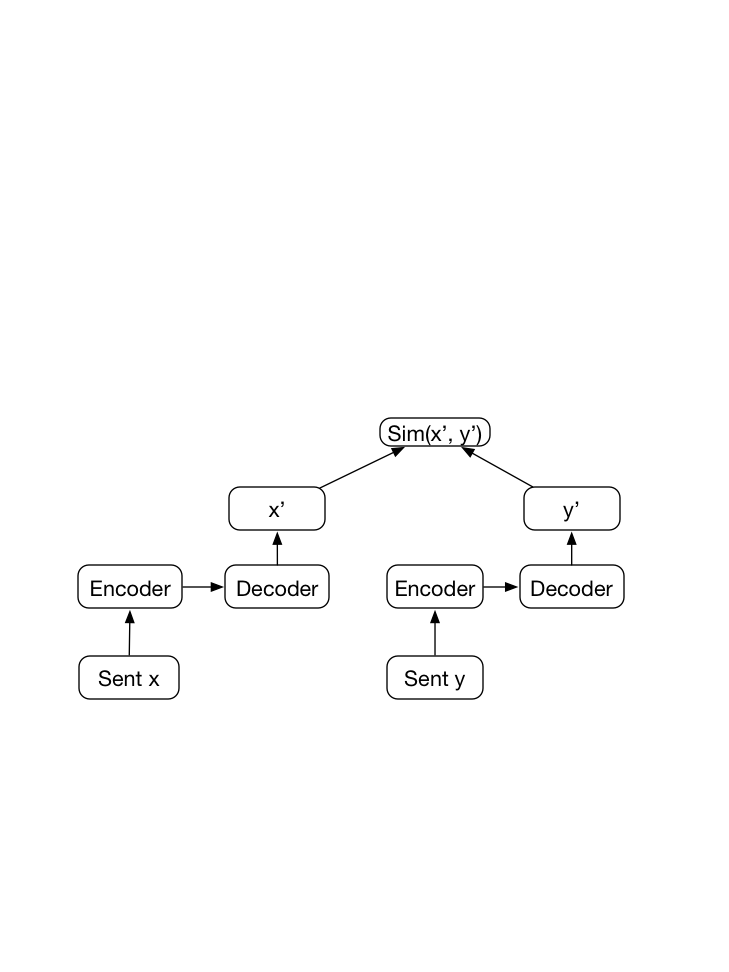
\includegraphics[width=0.7\linewidth]{model}
\caption{The structure of model}
\label{fig:model}
\end{figure}


The model includes two parts, one is normalization, and other is similarity.

The question that inspired this paper was whether neural language model could also benefit for text normalization.; that is ... To answer this question we introduce character-aware neural language model for tweets normalization.  \textbf{Draw the figure of model.}

\subsection{Long Short-Term Memory}
Recurrent neural networks (RNNs) are able to process input sequences of arbitrary length via the recursive application of a transition function on a hidden state vector \textit{$h_{t}$}. At each time step \textit{t}, the hidden state \textit{$h_{t}$} is a function of the input vector \textit{$x_{t}$} that the network receives at time \textit{t} and its previous hidden state \textit{$h_{t-1}$}. The hidden state \textit{$h_{t}$} $\in$ $\mathbf{R^{d}}$ can be interpreted as a \textit{d}-dimensional distributed representation of the sequence of tokens observed up to time \textit{t}. Commonly, the RNN transition function is an affine transformation followed by a pointwise non-linearity such as the hyperbolic tangent function:
\begin{equation}\label{rnn}
h_{t} = \tanh(Wx_{t}+Uh_{t-1}+b)
\end{equation}
However, a problem with RNNs with transition functions of this form is that during traning , components of the gradient vector can grow or decay exponentially over long sequences \cite{Hochreiter:1998:VGP:353515.355233}. This problem with exploding or vanishing gradients makes it difficult for the RNN model to learn long-distance correlations in a sequence.

The LSTM architecture addresses this problem of learning long-term dependencies by introducing a memory cell that is able to preserve state over long periods of time \cite{Hochreiter:1997:LSM:1246443.1246450}. While numerous LSTM variants have been described, here we describe the version used by Zaremba and Sutskever \shortcite{DBLP:journals/corr/ZarembaS14}. We define the LSTM unit at each time step \textit{t} to be a collection of vectors in \textbf{$R^{d}$}: an input gate \textit{$i_{t}$}, a forget gate \textit{$f_{t}$}, an output gate \textit{$o_{t}$}, a memory cell \textit{$c_{t}$} and a hidden state \textit{$h_{t}$}. The entries of the gating vectors \textit{$i_{t}$}, \textit{$f_{t}$} and \textit{$o_{t}$} are in [0, 1]. We refer to \textit{d} as the memory dimension of the LSTM. The LSTM transition equations are the following:
\begin{equation}\label{lstm-i}
i_{t} = \sigma(W^{(i)}x_{t}+U^{(i)}h_{t-1}+b^{(i)})
\end{equation}
\begin{equation}\label{lstm-f}
f_{t} = \sigma(W^{(f)}x_{t}+U^{(f)}h_{t-1}+b^{(f)})
\end{equation}
\begin{equation}\label{lstm-o}
o_{t} = \sigma(W^{(o)}x_{t}+U^{(o)}h_{t-1}+b^{(o)})
\end{equation}
\begin{equation}\label{lstm-u}
u_{t} = \tanh(W^{(u)}x_{t}+U^{(u)}h_{t-1}+b^{(u)})
\end{equation}
\begin{equation}\label{lstm-c}
c_{t} = i_{t} \odot u_{t} + f_{t} \odot c_{t-1}
\end{equation}
\begin{equation}\label{lstm-h}
h_{t} = o_{t} tanh(c_{t})
\end{equation}
where \textit{$x_{t}$} is the input at the current time step, $\sigma$ denotes the logistic sigmoid function and $\odot$ denotes elementwise multiplication. Intuitively, the forget gate controls the extent to which the previous memory cell is forgotten, the input gate controls how much each unit is updated, and the output gate controls the exposure of the internal memory state. The hidden state vector in an LSTM unit is therefore a gated, partial view of the state of the unit's internal memory cell. Since the value of the gating variables vary for each vector element, the model can learn to represent information over multiple time scales.

\subsection{Neural Language Model}
The goal of the LSTM is to estimate the conditional probability \textit{p}(\textit{$y_{1},...,y_{T^{'}}|x_{1},...,x_{T}$}) where (\textit{$x_{1},...,x_{T}$}) is an input sequence and \textit{$y_{1},...,y_{T^{'}}$} is its corresponding output sequence whose length \textit{$T^{'}$} may differ from \textit{T}. The LSTM computes this conditional probability by first obtaining the fixed-dimensional representation \textit{v} of the input sequence (\textit{$x_{1},...,x_{T}$}) given by the last hidden state of the LSTM, and then computing the probability of \textit{$y_{1},...,y_{T^{'}}$} with a standard LSTM language model formulation whose initial hidden state is set to the representation \textit{v} of \textit{$x_{1},...,x_{T}$}:
\begin{equation}\label{nlm}
p(y_{1},...,y_{T^{'}}|x_{1},...,x_{T})=\prod_{t=1}^{T^{'}}p(y_{t}|v,y_{1},...,y_{t-1})
\end{equation}
In this equation, each \textit{p($y_{t}|v,y_{1},...,y_{t-1}$)} distribution is represented with a softmax over all the words in the vocabulary. Note that we require that each sentence ends with a special end-of-sentence symbol ``$<$EOS$>$", which enables the model define a distribution over sequences of all possible lengths.

\subsection{Attention-Based Encoder }
Attention-based contextual encoder that constructs a representation based on the generation context. Attention models adopt a look-back strategy by linking the current decoding stage with input sentences in an attempt to consider which part of the input is most responsible for the current decoding state. 

Let \textit{H}= \{$h_{1}^{s}(e)$, $h_{2}^{s}(e)$, ..., $h_{N}^{s}(e)$\} be the collection of sentence-level hidden vectors for each sentence form the inputs, outputed from LSTM sentence encoder. Each element in \textit{H} contains information about input sequences with a strong focus on the parts surrounding each specific sentence (time-step). During decoding, suppose that \textit{$e_{t}^{s}$} denotes the sentence-level embedding at current step and that \textit{$h_{t-1}^{s}$}(dec) denotes the hidden vector outputted from LSTM sentence decode at previous time step \textit{t}-1. Attention models would first link the current step decoding information, i.e., \textit{$h_{t-1}^{s}$}(dec) which is outputted form LSTM with each of the input sentence \textit{i} $\in$ [1, \textit{N}], characterized by a strength indicator \textit{$v_{i}$}:
\begin{equation}\label{key}
v_{i} = U^{T}f(W_{1} \cdot h_{t-1}^{s}(dec) + W_{2} \cdot h_{i}^{s}(enc))
\end{equation}
\textit{$W_{1}$}, \textit{$W_{2}$} $\in$ $\mathbb{R}^{K \times K}$, \textit{U} $\in$ $\mathbb{R}^{K \times 1}$. \textit{$v_{i}$} is then normalized:
\begin{equation}\label{key}
a_{i}=\frac{\exp(v_{i})}{\sum_{i^{'}}\exp(v_{i}^{'})}
\end{equation}
The attention vector is then created by averaging weights over all input sentences:
\begin{equation}\label{key}
m_{t}=\sum_{i \in [1, N_{D}]}a_{i}h_{i}^{s}(enc)
\end{equation}
LSTM hidden vectors for current step is then achieved by combining \textit{$c_{t}$}, \textit{$e_{t}^{s}$} and \textit{$h_{t-1}^{s}$}(dec):

\begin{equation}\label{key}
c_{t} = f_{t} \cdot c_{t-1} + i_{t} \cdot l_{t}
\end{equation}
\begin{equation}\label{key}
h_{t}^{s} = o_{t} \cdot c_{t}
\end{equation}
where \textit{W} $\in$ $\mathbb{R}^{4K \times 3K}$. \textit{$h_{t}$} is then used for word predicting as in the vanilla version of the hierarchical model.

\subsection{Training}
The lack of generation constrants makes it posible to train the model on arbitrary input-output pairs. Once we have defined the local conditional model, \textit{$p$}($y_{i+1}$$|$x, $y_{c}$; $\theta$), we can estimate the parameters to minimize the negative log-likelihood of a set of summaries. Define this training set as consisting of \textit{N} input-output pairs ($\textbf{x}^{(1)}$, $\textbf{y}^{(1)}$),...,($\textbf{x}^{(N)}$, $\textbf{y}^{(N)}$). The negativ log-likelihood conveniently factors into a term for each token in the decode sentence:
\begin{equation}\label{key}
NLL(\theta)=-\sum_{j=1}^{J}\log p(\mathbf{y}^{(j)}|\mathbf{x}^{(j)};\theta)
\end{equation}
We minimize NLL by using mini-batch stochastic gradient descent.

\subsection{Attention}
In parallel, the concept of ``attention" has gained popularity recently in training neural networks, allowing models to learn alignments between different modalities. In the context of NMT, Bahdanaul et al. \shortcite{DBLP:journals/corr/BahdanauCB14} as successfully applied such attentional mechanism to jointly translate and align words. To the best of our knowledge, there has not been any other work exploring the use of attention-based architectures for NMT.

Word, Character, attention, sequence to sequence, language model, tweet normalization, semantic similarity, end-to-end.

\subsection{Normalization}
Given a piece of microtext, our model will normalize terms one bye one. Thus, the challenge is to determine the corresponding standard form \textit{t}, which can be a term or a sequence of terms, for each observed term \textit{t'}. Notice that \textit{t} many or may not be the same with \textit{t'}. \textit{t'} is a NSW if \textit{t'} $\neq$ \textit{t}. Thus, the task is to find the most probable normalization \textit{t*} for each observed term \textit{t'}:
\begin{equation}\label{key}
t*=argmax_{t}P(t|t')=argmax_{t}P(t'|t)P(t)
\end{equation}
P(t'$|$t) models the noisy channel through which an intended term \textit{t} is sent and is corrupted into the observed term \textit{t'}. P(t) models the source that generates the intended term \textit{t}. In practice, the source model can be approximated with an n-gram statistical language model.

Since a non-standard term and its corresponding standard form might be similar from one or multiple perspective(s), it is reasonable to assume that there are several channels, each of which would distort an intended term in one of the above aspects. More specifically, a grapheme channel would be responsible for the spelling distortion, a phoneme channel would cause phonetic corruptions, a context channel may shrink a sequence of terms into one term. In reality, an intended word may be transferred through one or multiple channels, and an observed term might be mixed corruption from more than one channel. Under this assumption, and letting \{\textit{$c_{k}$}$|$\textit{$c_{k} \in C$}\} denotes the set of channels, so the aforementioned equation can be further developed to 
\begin{equation}\label{key}
t*= argmax_{t}\sum_{k}P(t',c_{k}|t)P(t)
  = argmax_{t}\sum_{k}P(t'|c_{k},t)P(c_{k}|t)P(t)
\end{equation}
A term \textit{t} is transfered through channel \textit{$c_{k}$} with probability P($c_{k}|$t). Within the channel \textit{$c_{k}$}, term \textit{t} is distorted to term \textit{t}' according to the channel model P(t'$|c_{k}$, t).

Many approaches to text normalization adopt the noisy channel setting, where the model normalization source sentence \textit{s} into target canonical form \textit{t} is factored into two parts $\hat{t}$ = argmax$_{t}$\textit{P}(\textit{t})\textit{P}(\textit{s}$\vert$\textit{t}). The error term \textit{P}(\textit{s}$\vert$\textit{t}) models hwo canonical strings are transformed into variants such as misspellings or abbreviations. The language model \textit{P}(\textit{t}) encodes which target strings are probable. When large-scale normalized texts have been trained with language model, the weights of the model are obtained with the normalization corpus. When the informal texts are inputed into model, the decoder of the proposed model will output the normalized text sequence and the informall words will be changed following the context information, which will be expressed with normalized words form normalized corpus dictionary. \textbf{AAAI2011Normalizing Microtext}

\subsection{Similarity Measurement}
We adopt a siamese architecture for learning sentence similarity. There are two networks LSTM$_a$ and LSTM$_b$ which each process one of the sentences in a given pair, but our networks architecture tied weights such that LSTM$_a$ equals LSTM$_b$ in this work. Nevertheless, the general united version of this model may be more useful for applications with asymmetric domains such as information retrieval. The LSTM learns a mapping from the space of variable length sequences of d$_in$-dimensional vectors into $\mathbb{R}^{d_{rep}}$. More concretely, each sentence (represented as a sequence of word vectors) \textit{$x_{1},\cdots,x_{T}$}, is passed to the LSTM, which updates its hidden state at each sequence-index. The final representation of the sentence is encoded by \textit{$h_{T}$} $\in$ $\mathbb{R}^{d_{rep}}$, 
the last hidden state of the model. For a given pair of sentences, our approach applies a pre-defined similarity function \textit{g}: $\mathbb{R}^{d_{rep}}\times\mathbb{R}^{d_{rep}}\rightarrow\mathbb{R}$ to their LSTM-representations. Similarites in the representation space are subsequently used to infer the sentences' underlying semantic similarity.

Note that unlike typical language model RNNs, which are used to predict the next word given the previous text, our LSTMs simply function like the encoder of sequence to sequence model. Thus, the sole error signal backpropagated during training stems from the similarity between sentence representations \textit{$h_{T_{a}}^{(a)}$}, \textit{$h_{T_{b}}^{(b)}$}, and how this predicted similarity deviate from the human annotated ground truth relatedness. We restrict ourselves to the simple similarity function: (\textit{subscript must be changed as $h_{T_{1}}^{(1)}$}, or it is same as SiamStru(AAAI16).)
\begin{equation}\label{key}
sim(h_{T_{a}}^{(a)},h_{T_{b}}^{(b)}) = \exp(-||h_{T_{a}}^{(a)}-h_{T_{b}}^{(b)}||_{1}) \in [0,1]
\end{equation}
This forces the LSTM to entirely capture the semantic difference during training, rather than supplementing the RNN with a more complex learner that can help resolve shorcoming in the learned representations.

\section{Experiments}
We evaluated our model on the tweet normalization and paraphrase identification task, which is a benchmark for evaluating many semantic similarity models.

\subsection{Dataset}
The following data sets are used in our experiments. It includes tweet normalization and paraphrase identification.

\begin{itemize}
	\item Data 1: 2,333 unique pairs of informal tokens and normalized words, collected form 2,577 Twitter messages, which selected form the Edinburgh Twitter corpus \cite{pennell-liu:2011:IJCNLP-2011}. And some changes were made on this data\footnote{http://www.hlt.utdallas.edu/~chenli/normalization} by Li and Yang \shortcite{li-liu:2014:P14-3}. This data is used for training the normalization models for tweet normalization.
	\item Data 2: The data\footnote{http://www.hlt.utdallas.edu/~chenli/normalization\underline{ }pos/} was created by Chen and Liu \shortcite{Li:2015:JPT:2832415.2832425}, which is used for joint POS tagging and normalization of non-standard tokens. The data contains two parts: one is from, which includes 549 tweets. The another contains 789 tweets. We removed the POS tagging and use the first as development data and the second as test data.
	\item Data 3: We use the PIT corpus\footnote{http://www.cis.upenn.edu/~xwe/
	semeval2015pit/} for evaluating paraphrase identification. The training and development set contain 17,790 sentence pairs and test set includes 972 sentence pairs\cite{xu-callisonburch-dolan:2015:SemEval}. The data set can be used for paraphrase identification and semantic similarity in Twitter.
\end{itemize}

\subsection{Traing Detail}
Existing research has shown that attention mechanism work better than shallow recurrent neural network for squence to sequence tasks \cite{luong-pham-manning:2015:EMNLP,Sutskever:2014:SSL:2969033.2969173}. We adopt attention-based end-to-end structure with three layer for encoding and three layer for decoding, each of which is comprised of a different set of parameters. Each LSTM layers consists of 500 hidden neurons and the dimensionality of word embeddings is set to 500. Some other training details given as following.

\begin{itemize}	
	\item Input sentence sequences are reversed.
	\item Parameters are initialized form a uniform distribution between [-0.1, 0.1].
	\item Batch size is set to 16.
	\item Stochastic gradient descent is implemented without momentum using a fixed learning rate of 1. We start halving the learning rate every half epoch after 5 epochs. We trained our models for a total of 20 epoches.
	\item Dropout rate is set to 0.3.
	\item Size of the character embeddings is set to 30.
	\item Number of covolution filters is 500.
\end{itemize}

Our implementation on a single GPU\footnote{The GPUs with 1280 Cuda cores and 6GB memory.} processes a speed of approximately 5,000-6,000 tokens per second.

\subsection{Tweet Normalization}
We 

\subsection{Paraphrase Detection}

\section{Related Work}
Neural language models (NLM) contain a rich family of neural network architectures for language modeling. Some examples encompass recurrent \cite{mikolov2010recurrent}, convolutional \cite{wang-EtAl:2015:ACL-IJCNLP3}, and convolutional-recurrent \cite{Kim-AAAI1612489}. In Twitter, there are existing rare and unknown words due to the social media characteristic,  therefore it is necessary for language model to point the unknown words before normalization. A neural network models using attention adopted two softmax layers in order to predict the next word in conditional language models \cite{gulcehre-EtAl:2016:P16-1}. Recurrent memory network \cite{tran-bisazza-monz:2016:N16-1} not only amplifies the power of recurrent neural networks but also facilitates the understanding of its internal functions, the model can learn the correct words by the trained language model. Log-bilinear language models integrate compositional morphological representations and probabilistic language modelling \cite{jan-phil:2014:icml}.

Character-aware neural language model \cite{Kim-AAAI1612489} can capture morphological features based on character-level input and the output is still word-level. Because the social media has long-tailed frequency distributions or domains with dynamic vocabularies, so the model can leverage subword information for tweets normalization. The existing works for semantic similarity focus on sequence representation, and the model structure is usually a siamese architecture, which represent sentence pairs and compute the semantic similarity between pairs \cite{jonas-aditya:2016:AAAI}. Convolutional neural networks are used for representing sentence and learn multigranular sentence representations for paraphrase identification was proposed \cite{yin-schutze:2015:NAACL}. The deep learning architecture based on convolutional networks can obtain mutliple levels of granularity, including unigram, short-ngram, long-ngram and sentence-level features, which are computed for similarity comparation for paraphrase detection.

Although normalization on informal text has potential function on sentence representation and semantic similarity, paraphrase can also improve the normalization performance \cite{ling-EtAl:2013:EMNLP} on parallel microblog data. Applying alignment feature for semantic similarity of text can capture both local ifnormation like lexical semantics and structural information like syntactic structures \cite{chen-praveen:2016:ijcai}. The method can avoid conventional fixed-length sentence representation and add more feature information for similarity measurement. Some works \cite{DBLP:journals/corr/WietingBGL15a,pavlick-EtAl:2015:ACL-IJCNLP} consider the utilization of paraphrse database \cite{ganitkevitch-vandurme-callisonburch:2013:NAACL-HLT,pavlick-EtAl:2015:ACL-IJCNLP3}for sentence similarity, entialment, and sentiment classification.

Our work apply character-level input style convolutional recurrent neural network model for trianing a language model on word-level prediction. After pre-trained with formal corpus such as Wiki or Penn Treebank data, the language model is used for normalizing the informal tweets, which can automatically point unknown or non-standard words and normalize them. The normalized tweets will be measured semantic similarity further, and the similarity will feedback for normalization based on assumptaion that paraphrasing sentence pairs will keep semantic equivalence. The experimental results demonstrate that our model outperform the existing state-of-the-art systems.

\section{Conclusion}
We accomplished a model and obtain a higher performance. In the future, we will do more works. We are going to use language model for normalization using the character-aware model. And paraphrase identification tasks are used for evaluating the performance of normalization in tweets.About tweet similarity, including paraphrase identification and entialment etc.. Moreover, the key work is about normalization in tweets. We are going to use language model for normalization using the character-aware model. And paraphrase identification tasks are used for evaluating the performance of normalization in tweets. We accomplished a model and obtain a higher performance. In the future, we will do more works. We are going to use language model for normalization using the character-aware model. And paraphrase identification tasks are used for evaluating the performance of normalization in tweets.About tweet similarity, including paraphrase identification and entialment etc.. Moreover, the key work is about normalization in tweets. We are going to use language model for normalization using the character-aware model. And paraphrase identification tasks are used for evaluating the performance of normalization in tweets.

\bibliographystyle{aaai}
\bibliography{aaai16.bib}





\noindent Congratulations on having a paper selected for inclusion in an AAAI Press proceedings or technical report! This document details the requirements necessary to get your accepted paper published using \LaTeX{}. If you are using Microsoft Word, instructions are provided in a different document. If you want to use some other formatting software, you must obtain permission from AAAI Press first. 

The instructions herein are provided as a general guide for experienced \LaTeX{} users who would like to use that software to format their paper for an AAAI Press publication or report. If you are not an experienced \LaTeX{} user, do not use it to format your paper. AAAI cannot provide you with support and the accompanying style files are \textbf{not} guaranteed to work. If the results you obtain are not in accordance with the specifications you received, you must correct your source file to achieve the correct result. 

These instructions are generic. Consequently, they do not include specific dates, page charges, and so forth. Please consult your specific written conference instructions for details regarding your submission. Please review the entire document for specific instructions that might apply to your particular situation. All authors must comply with the following:

\begin{itemize}
\item You must use the latest AAAI Press \LaTeX{} macro.
\item Download the author kit.
\item Complete, sign, and return by the deadline the AAAI copyright form (proceedings authors) or distribution license (technical report authors).
\item Read and format your paper source and PDF according to the formatting instructions for authors.
\item Submit your electronic files and abstract using our electronic submission form \textbf{on time.}
\item Submit your copyright form, and any required page or formatting charges to AAAI Press so that they are received by the deadline.
\item Check every page of your paper before submitting it.
\end{itemize}

\section{Copyright}
All papers submitted for publication by AAAI Press must be accompanied by a valid signed copyright form or, in the case of technical reports, by a valid signed permission to distribute form. There are no exceptions to this requirement. You must send us the original version of this form. However, to meet the deadline, you may fax (1-650-321-4457) or scan and e-mail the form (pubforms16@aaai.org) to AAAI by the submission deadline, and then mail the original via postal mail to the AAAI office. \textbf{If you fail to send in a signed copyright or permission form, your paper will not be published.} You will find PDF versions of the AAAI copyright and permission to distribute forms in the author kit.

\section{Formatting Requirements in Brief}
We need source and PDF files that can be used in a variety of ways and can be output on a variety of devices. AAAI imposes some requirements on your source and PDF files that must be followed. Most of these requirements are based on our efforts to standardize conference manuscript properties and layout. These requirements are as follows, and all papers submitted to AAAI for publication must comply:

\begin{itemize}
\item Your .tex file must compile in PDF\LaTeX{} --- \textbf{ no .ps or .eps figure files.}
\item All fonts must be embedded in the PDF file --- \textbf{ this includes your figures.}
\item Modifications to the style sheet (or your document) in an effort to avoid extra page charges are NOT allowed.
\item No type 3 fonts may be used (even in illustrations).
\item Your title must follow Title Case capitalization rules (not sentence case).
\item \LaTeX{} documents must use the Times or Nimbus font package (do not use Computer Modern for the text of your paper).
\item No \LaTeX{} 209 documents may be used or submitted.
\item Fonts that require non-English language support (CID and Identity-H) must be converted to outlines or removed from the document (even if they are in a graphics file embedded in the document). 
\item Two-column format in AAAI style is required for all papers.
\item The paper size for final submission must be US letter. No exceptions.
\item The source file must exactly match the PDF.
\item The document margins must be as specified in the formatting instructions.
\item The number of pages and the file size must be as specified for your event.
\item No document may be password protected.
\item Neither the PDFs nor the source may contain any embedded links or bookmarks.
\item Your source and PDF must not have any page numbers, footers, or headers.
\item Your PDF must be compatible with Acrobat 5 or higher.
\item Your \LaTeX{} source file (excluding references) must consist of a \textbf{single} file (use of the ``input" command is not allowed.
\item Your graphics must be sized appropriately outside of \LaTeX{} (do not use the ``clip" command) .
\end{itemize}

If you do not follow the above requirements, it is likely that we will be unable to publish your paper.

\section{What Files to Submit}
You must submit the following items to ensure that your paper is published:
\begin{itemize}
\item A fully-compliant PDF file.
\item Your  \LaTeX{}  source file submitted as a \textbf{single} .tex file (do not use the ``input" command to include sections of your paper --- every section must be in the single source file). The only exception is the bibliography, which you may include separately. Your source must compile on our system, which includes the standard \LaTeX{} support files.
\item All your graphics files.
\item The \LaTeX{}-generated files (e.g. .aux and .bib file, etc.) for your compiled source.
\item All the nonstandard style files (ones not commonly found in standard \LaTeX{} installations) used in your document (including, for example, old algorithm style files). If in doubt, include it.
\end{itemize}

Your \LaTeX{} source will be reviewed and recompiled on our system (if it does not compile, you may incur late fees).   \textbf{Do not submit your source in multiple text files.} Your single \LaTeX{} source file must include all your text, your bibliography (formatted using aaai.bst), and any custom macros. Accompanying this source file, you must also supply any nonstandard (or older) referenced style files and all your referenced graphics files. 

Your files should work without any supporting files (other than the program itself) on any computer with a standard \LaTeX{} distribution. Place your PDF and source files in a single tar, zipped, gzipped, stuffed, or compressed archive. Name your source file with your last (family) name.

\textbf{Do not send files that are not actually used in the paper.} We don't want you to send us any files not needed for compiling your paper, including, for example, this instructions file, unused graphics files, and so forth.  A shell script (created by an AAAI member --- it might not work without modification on your system) that might help you create the \LaTeX{} source package is included in the Author Kit.

\section{Using \LaTeX{} to Format Your Paper}

The latest version of the AAAI style file is available on AAAI's website. Download this file and place it in a file named ``aaai.sty" in the \TeX\ search path. Placing it in the same directory as the paper should also work. You must download the latest version of the complete author kit so that you will have the latest instruction set.

\subsection{Document Preamble}

In the \LaTeX{} source for your paper, you \textbf{must} place the following lines as shown in the example in this subsection. This command set-up is for three authors. Add or subtract author and address lines as necessary, and uncomment the portions that apply to you. In most instances, this is all you need to do to format your paper in the Times font. The helvet package will cause Helvetica to be used for sans serif, and the courier package will cause Courier to be used for the typewriter font. These files are part of the PSNFSS2e package, which is freely available from many Internet sites (and is often part of a standard installation).

Leave the setcounter for section number depth commented out and set at 0 unless you want to add section numbers to your paper. If you do add section numbers, you must uncomment this line and change the number to 1 (for section numbers), or 2 (for section and subsection numbers). The style file will not work properly with numbering of subsubsections, so do not use a number higher than 2.


\begin{quote}
\begin{small}
\textbackslash documentclass[letterpaper]{article}\\
\% \textit{Required Packages}\\
\textbackslash usepackage\{aaai\}\\
\textbackslash usepackage\{times\}\\
\textbackslash usepackage\{helvet\}\\
\textbackslash usepackage\{courier\}\\
\textbackslash setlength\{\textbackslash pdfpagewidth\}\{8.5in\}
\textbackslash setlength\{\textbackslash pdfpageheight\}\{11in\}\\
\%\%\%\%\%\%\%\%\%\%\\
\% \textit{PDFINFO for PDF\LaTeX{}}\\
\% Uncomment and complete the following for metadata (your paper must compile with PDF\LaTeX{})\\
\textbackslash pdfinfo\{\\
/Title (Input Your Paper Title Here)\\
/Author (John Doe, Jane Doe)\\
/Keywords (Input your paper's keywords in this optional area)\\
\}\\
\%\%\%\%\%\%\%\%\%\%\\
\% \textit{Section Numbers}\\
\% Uncomment if you want to use section numbers\\
\% and change the 0 to a 1 or 2\\
\% \textbackslash setcounter\{secnumdepth\}\{0\}\\
\%\%\%\%\%\%\%\%\%\%\\
\% \textit{Title, Author, and Address Information}\\
\textbackslash title\{Title\}\\
\textbackslash author\{Author 1 \textbackslash and Author 2\textbackslash\textbackslash \\ 
Address line\textbackslash\textbackslash\\ Address line\textbackslash\textbackslash \\
\textbackslash And\\
Author 3\textbackslash\textbackslash\\ Address line\textbackslash\textbackslash\\ Address line\}\\
\%\%\%\%\%\%\%\%\%\%\\
\% \textit{Body of Paper Begins}\\
\textbackslash begin\{document\}\\
\textbackslash maketitle\\
...\\
\%\%\%\%\%\%\%\%\%\%\\
\% \textit{References and End of Paper}\\
\textbackslash bibliography\{Bibliography-File\}\\
\textbackslash bibliographystyle\{aaai\}\\
\textbackslash end\{document\}
\end{small}
\end{quote}

\subsection{Inserting Document Metadata with \LaTeX{}}
PDF files contain document summary information that enables us to create an Acrobat index (pdx) file, and also allows search engines to locate and present your paper more accurately. \textbf{Document Metadata  for Author and Title are REQUIRED.} 

If your paper includes illustrations that are not compatible with PDF\TeX{} (such as .eps or .ps documents), you will need to convert them. The epstopdf package will usually work for eps files. You will need to convert your ps files to PDF however.

\textit{Important:} Do not include \textit{any} \LaTeX{} code or nonascii characters (including accented characters) in the metadata. The data in the metadata must be completely plain ascii. It may not include slashes, accents, linebreaks, unicode, or any \LaTeX{} commands. Type the title exactly as it appears on the paper (minus all formatting). Input the author names in the order in which they appear on the paper (minus all accents), separating each author by a comma. You may also include keywords in the Keywords field.



\subsection{Preparing Your Paper}

After the preamble above, you should prepare your paper as follows:

\begin{quote}
\begin{small}
\textbackslash begin\{document\}\\
\textbackslash maketitle\\
...\\
\textbackslash bibliography\{Bibliography-File\}\\
\textbackslash bibliographystyle\{aaai\}\\
\textbackslash end\{document\}\\
\end{small}
\end{quote}
\subsection{Incompatible Packages}
The following packages are incompatible with aaai.sty and/or aaai.bst and must not be used (this list is not exhaustive --- there are others as well):
\begin{itemize}
\item authblk
\item fullpage
\item hyperref
\item natbib
\item geometry
\item titlesec
\item layout
\item caption
\item titlesec
\item savetrees
\item T1 fontenc package (install the CM super fonts package instead)
\end{itemize}

\subsection{Illegal Commands}
The following commands may not be used in your paper (this list is exhaustive --- there are others; generally, if it alters aaai.sty, it isn't acceptable):
\begin{itemize}
\item \textbackslash input
\item \textbackslash vspace or vskip (when used before or after a section or subsection)
\item \textbackslash addtolength 
\item \textbackslash columnsep
\item \textbackslash top margin (or text height or addsidemargin or even side margin)
\item trim or clip (used to crop figures)
\item any command that globally alters floats, space above and below figures and tables
\end{itemize}

\subsection{Paper Size, Margins, and Column Width}
Papers must be formatted to print in two-column format on 8.5 x 11 inch US letter-sized paper. The margins must be exactly as follows: 
\begin{itemize}
\item Top margin: .75 inches
\item Left margin: .75 inches
\item Right margin: .75 inches
\item Bottom margin: 1.25 inches
\end{itemize} 


The default paper size in most installations of \LaTeX{} is A4. However, because we require that your electronic paper be formatted in US letter size, you will need to alter the default for this paper to US letter size. Assuming you are using the 2e version of \LaTeX{}, you can do this by including the [letterpaper] option at the beginning of your file: 
\textbackslash documentclass[letterpaper]{article}. 

This command is usually sufficient to change the format. Sometimes, however, it may not work. Use PDF\LaTeX{} and include
\textbackslash setlength\{\textbackslash pdfpagewidth\}\{8.5in\}
\textbackslash setlength\{\textbackslash pdfpageheight\}\{11in\}
in your preamble. 

\textbf{Do not use the Geometry package to alter the page size.} Use of this style file alters aaai.sty and will result in your paper being rejected. 


\subsubsection{Column Width and Margins.}
To ensure maximum readability, your paper must include two columns. Each column should be 3.3 inches wide (slightly more than 3.25 inches), with a .375 inch (.952 cm) gutter of white space between the two columns. The aaai.sty file will automatically create these columns for you. 

\subsection{Overlength Papers}
If your paper is too long, turn on \textbackslash frenchspacing, which will reduce the space after periods. Next,  shrink the size of your graphics. Use \textbackslash centering instead of \textbackslash begin\{center\} in your figure environment. For mathematical environments, you may minimally reduce \textbackslash abovedisplayskip, \textbackslash belowdisplayskip, and \textbackslash arraycolsep. You may also alter the size of your bibliography by inserting \textbackslash fontsize\{9.5pt\}\{10.5pt\} \textbackslash selectfont
right before the bibliography (the minimum size is \textbackslash fontsize\{9.0pt\}\{10.0pt\}. 

Commands that alter page layout are forbidden. These include \textbackslash columnsep, \textbackslash topmargin, \textbackslash topskip, \textbackslash textheight, \textbackslash textwidth, \textbackslash oddsidemargin, and \textbackslash evensizemargin (this list is not exhaustive). If you alter page layout, you will be required to pay the page fee \textit{plus} a reformatting fee. Other commands that are questionable and may cause your paper to be rejected include  \textbackslash parindent, and \textbackslash parskip. Commands that alter the space between sections are also questionable. The title sec package is not allowed. Regardless of the above, if your paper is obviously ``squeezed" it is not going to to be accepted. Before using every trick you know to make your paper a certain length, try reducing the size of your graphics or cutting text instead or (if allowed) paying the extra page charge. It will be cheaper in the long run.

\subsection{Figures}
Your paper must compile in PDF\LaTeX{}. Consequently, all your figures must be .jpg, .png, or .pdf. You may not use the .gif (the resolution is too low), .ps, or .eps file format for your figures.

When you include your figures, you must crop them \textbf{outside} of \LaTeX{}. The command \textbackslash includegraphics*[clip=true, viewport 0 0 10 10]{...} might result in a PDF that looks great, but the image is \textbf{not really cropped.} The full image can reappear (and obscure whatever it is overlapping) when page numbers are applied or color space is standardized. 

\subsection{Type Font and Size}
Your paper must be formatted in Times Roman or Nimbus. We will not accept papers formatted using Computer Modern or Palatino or some other font as the text or heading typeface. Sans serif, when used, should be Courier. Use Symbol or Lucida or Computer Modern for \textit{mathematics only. } 

Do not use type 3 fonts for any portion of your paper, including graphics. Type 3 bitmapped fonts are designed for fixed resolution printers. Most print at 300 dpi even if the printer resolution is 1200 dpi or higher. They also often cause high resolution imagesetter devices and our PDF indexing software to crash. Consequently, AAAI will not accept electronic files containing obsolete type 3 fonts. Files containing those fonts (even in graphics) will be rejected. 

Fortunately, there are effective workarounds that will prevent your file from embedding type 3 bitmapped fonts. The easiest workaround is to use the required times, helvet, and courier packages with \LaTeX{}2e. (Note that papers formatted in this way will still use Computer Modern for the mathematics. To make the math look good, you'll either have to use Symbol or Lucida, or you will need to install type 1 Computer Modern fonts --- for more on these fonts, see the section ``Obtaining Type 1 Computer Modern.")

If you are unsure if your paper contains type 3 fonts, view the PDF in Acrobat Reader. The Properties/Fonts window will display the font name, font type, and encoding properties of all the fonts in the document. If you are unsure if your graphics contain type 3 fonts (and they are PostScript or encapsulated PostScript documents), create PDF versions of them, and consult the properties window in Acrobat Reader. 

The default size for your type should be ten-point with twelve-point leading (line spacing). Start all pages (except the first) directly under the top margin. (See the next section for instructions on formatting the title page.) Indent ten points when beginning a new paragraph, unless the paragraph begins directly below a heading or subheading.

\subsubsection{Obtaining Type 1 Computer Modern for \LaTeX{}.}

If you use Computer Modern for the mathematics in your paper (you cannot use it for the text) you may need to download type 1 Computer fonts. They are available without charge from the American Mathematical Society:
http://www.ams.org/tex/type1-fonts.html. 

\subsection{Title and Authors}
Your title must appear in mixed case (nouns, pronouns, and verbs are capitalized) near the top of the first page, centered over both columns in sixteen-point bold type (twenty-four point leading). This style is called ``mixed case." Author's names should appear below the title of the paper, centered in twelve-point type (with fifteen point leading), along with affiliation(s) and complete address(es) (including electronic mail address if available) in nine-point roman type (the twelve point leading). (If the title is long, or you have many authors, you may reduce the specified point sizes by up to two points.) You should begin the two-column format when you come to the abstract. 

\subsubsection{Formatting Author Information}
Author information can be set in a number of different styles, depending on the number of authors and the number of affiliations you need to display. For several authors from the same institution, use \textbackslash and:

\begin{quote}
\begin{small}
\textbackslash author\{Author 1 \textbackslash and  ...  \textbackslash and Author \textit{n}\textbackslash \textbackslash  \\
Address line \textbackslash \textbackslash ~... \textbackslash \textbackslash ~Address line\}
\end{small}
\end{quote}

\noindent If the names do not fit well on one line use:

\begin{quote}
\begin{small}
\textbackslash author\{Author 1\}\textbackslash \textbackslash \\ \{\textbackslash bf Author 2\}\textbackslash \textbackslash ~ 
... \textbackslash \textbackslash ~\{\textbackslash bf Author \textit{n}\}\textbackslash \textbackslash \\
Address line \textbackslash \textbackslash ~ ... \textbackslash \textbackslash ~ Address line\}
\end{small}
\end{quote}

\noindent For authors from different institutions, use \textbackslash And:

\begin{quote}
\begin{small}
\textbackslash author\{Author 1\textbackslash \textbackslash ~ Address line \textbackslash \textbackslash ~...  \textbackslash \textbackslash ~ Address line
\textbackslash And  ...  
\textbackslash And
Author \textit{n}\textbackslash \textbackslash \\ Address line\textbackslash \textbackslash ~
... \textbackslash \textbackslash ~
Address line\}
\end{small}
\end{quote}

\noindent To start a separate ``row" of authors, use \textbackslash AND:
\begin{quote}
\begin{small}
\textbackslash author\{Author 1\textbackslash\textbackslash ~ Address line \textbackslash\textbackslash ~
...  \textbackslash \textbackslash ~ Address line\textbackslash\textbackslash \\
\textbackslash AND\\
Author 2 \textbackslash\textbackslash ~ Address line \textbackslash\textbackslash ~
...  \textbackslash \textbackslash ~ Address line\textbackslash\textbackslash \\
\textbackslash And\\
Author 3 \textbackslash\textbackslash ~ Address line \textbackslash\textbackslash ~
...  \textbackslash \textbackslash ~ Address line\textbackslash\textbackslash \\\}
\end{small}
\end{quote}

\noindent If the title and author information does not fit in the area allocated, place
\textbackslash setlength\textbackslash titlebox\{\textit{height}\}
after the \textbackslash documentclass line where \{\textit{height}\} is something like 2.5in.

\subsection{\LaTeX{} Copyright Notice}
The copyright notice automatically appears if you use aaai.sty. If you are creating a technical report, it is not necessary to include this notice. You may disable the copyright line using the \verb+\+nocopyrightcommand. To change the entire text of the copyright slug, use:
\textbackslash copyrighttext \{\emph{text}\}.
Either of these must appear before \textbackslash maketitle. Please be advised, however, that \textit{if you disable or change the copyright line and transfer of copyright is required, your paper will not be published.}

\subsection{Credits}
Any credits to a sponsoring agency should appear in the acknowledgments section, unless the agency requires different placement. If it is necessary to include this information on the front page, use
\textbackslash thanks in either the \textbackslash author or \textbackslash title commands.
For example:
\begin{quote}
\begin{small}
\textbackslash title\{Very Important Results in AI\textbackslash thanks\{This work is
 supported by everybody.\}\}
\end{small}
\end{quote}
Multiple \textbackslash thanks commands can be given. Each will result in a separate footnote indication in the author or title with the corresponding text at the botton of the first column of the document. Note that the \textbackslash thanks command is fragile. You will need to use \textbackslash protect.

Please do not include \textbackslash pubnote commands in your document.

\subsection{Abstract}
The abstract must be placed at the beginning of the first column, indented ten points from the left and right margins. The title �Abstract� should appear in ten-point bold type, centered above the body of the abstract. The abstract should be set in nine-point type with ten-point leading. This concise, one-paragraph summary should describe the general thesis and conclusion of your paper. A reader should be able to learn the purpose of the paper and the reason for its importance from the abstract. The abstract should be no more than two hundred words in length. (Authors who are submitting short one- or two-page extended extracts should provide a short abstract of only a sentence or so.) \textbf{Do not include references in your abstract!}

\subsection{Page Numbers}

Do not \textbf{ever} print any page numbers on your paper. 

\subsection{Text }
The main body of the paper must be formatted in ten-point with twelve-point leading (line spacing).

\subsection{Citations}
Citations within the text should include the author's last name and year, for example (Newell 1980). Append lower-case letters to the year in cases of ambiguity. Multiple authors should be treated as follows: (Feigenbaum and Engelmore 1988) or (Ford, Hayes, and Glymour 1992). In the case of four or more authors, list only the first author, followed by et al. (Ford et al. 1997).

\subsection{Extracts}
Long quotations and extracts should be indented ten points from the left and right margins. 

\begin{quote}
This is an example of an extract or quotation. Note the indent on both sides. Quotation marks are not necessary if you offset the text in a block like this, and properly identify and cite the quotation in the text. 

\end{quote}

\subsection{Footnotes}
Avoid footnotes as much as possible; they interrupt the reading of the text. When essential, they should be consecutively numbered throughout with superscript Arabic numbers. Footnotes should appear at the bottom of the page, separated from the text by a blank line space and a thin, half-point rule. 

\subsection{Headings and Sections}
When necessary, headings should be used to separate major sections of your paper. Remember, you are writing a short paper, not a lengthy book! An overabundance of headings will tend to make your paper look more like an outline than a paper.

First-level heads should be twelve-point Times Roman bold type, mixed case (initial capitals followed by lower case on all words except articles, conjunctions, and prepositions, which should appear entirely in lower case), with fifteen-point leading, centered, with one blank line preceding them and three additional points of leading following them. Second-level headings should be eleven-point Times Roman bold type, mixed case, with thirteen-point leading, flush left, with one blank line preceding them and three additional points of leading following them. Do not skip a line between paragraphs. Third-level headings should be run in with the text, ten-point Times Roman bold type, mixed case, with twelve-point leading, flush left, with six points of additional space preceding them and no additional points of leading following them.

\subsubsection{Section Numbers}
The use of section numbers in AAAI Press papers is optional. To use section numbers in \LaTeX{}, uncomment the setcounter line in your document preamble and change the 0 to a 1 or 2. Section numbers should not be used in short poster papers.

\subsubsection{Section Headings.}
Sections should be arranged and headed as follows: 

\subsubsection{Acknowledgments.}
The acknowledgments section, if included, appears after the main body of text and is headed ``Acknowledgments." This section includes acknowledgments of help from associates and colleagues, credits to sponsoring agencies, financial support, and permission to publish. Please acknowledge other contributors, grant support, and so forth, in this section. Do not put acknowledgments in a footnote on the first page. If your grant agency requires acknowledgment of the grant on page 1, limit the footnote to the required statement, and put the remaining acknowledgments at the back. Please try to limit acknowledgments to no more than three sentences. 

\subsubsection{Appendices.}
Any appendices follow the acknowledgments, if included, or after the main body of text if no acknowledgments appear. 

\subsubsection{References}
The references section should be labeled ``References" and should appear at the very end of the paper (don't end the paper with references, and then put a figure by itself on the last page). A sample list of references is given later on in these instructions. Please use a consistent format for references. Poorly prepared or sloppy references reflect badly on the quality of your paper and your research. Please prepare complete and accurate citations.

\subsection{Illustrations and Figures}
Figures, drawings, tables, and photographs should be placed throughout the paper near the place where they are first discussed. Do not group them together at the end of the paper. If placed at the top or bottom of the paper, illustrations may run across both columns. Figures must not invade the top, bottom, or side margin areas. Figures must be inserted using the \textbackslash usepackage\{graphicx\}. Number figures sequentially, for example, figure 1, and so on. 

The illustration number and caption should appear under the illustration. Labels, and other text in illustrations must be at least nine-point type. 

\subsubsection{Low-Resolution Bitmaps.}
You may not use low-resolution (such as 72 dpi) screen-dumps and GIF files---these files contain so few pixels that they are always blurry, and illegible when printed. If they are color, they will become an indecipherable mess when converted to black and white. This is always the case with gif files, which should never be used. The resolution of screen dumps can be increased by reducing the print size of the original file while retaining the same number of pixels. You can also enlarge files by manipulating them in software such as PhotoShop. Your figures should be a minimum of 266 dpi when incorporated into your document.

\subsubsection{\LaTeX{} Overflow.}
\LaTeX{} users please beware: \LaTeX{} will sometimes put portions of the figure or table or an equation in the margin. If this happens, you need to scale the figure or table down, or reformat the equation. Check your log file! You must fix any overflow into the margin (that means no overfull boxes in \LaTeX{}). If you don't, the overflow text will simply be eliminated. \textbf{Nothing is permitted to intrude into the margins.}

\subsubsection{Using Color.}
Your paper will be printed in black and white and grayscale. Consequently, because conversion to grayscale can cause undesirable effects (red changes to black, yellow can disappear, and so forth), we strongly suggest you avoid placing color figures in your document. Of course, any reference to color will be indecipherable to your reader. 

\subsubsection{Drawings.}
We suggest you use computer drawing software (such as Adobe Illustrator or, (if unavoidable), the drawing tools in Microsoft Word) to create your illustrations. Do not use Microsoft Publisher. These illustrations will look best if all line widths are uniform (half- to two-point in size), and you do not create labels over shaded areas. Shading should be 133 lines per inch if possible. Use Times Roman or Helvetica for all figure call-outs. \textbf{Do not use hairline width lines} --- be sure that the stroke width of all lines is at least .5 pt. Zero point lines will print on a laser printer, but will completely disappear on the high-resolution devices used by our printers.

\subsubsection{Photographs and Images.}
Photographs and other images should be in grayscale (color photographs will not reproduce well; for example, red tones will reproduce as black, yellow may turn to white, and so forth) and set to a minimum of 266 dpi. Do not prescreen images.

\subsubsection{Resizing Graphics.}
Resize your graphics \textbf{before} you include them with LaTeX. You may \textbf{not} use trim or clip options as part of your \textbackslash includgraphics command. Resize the media box of your PDF using a graphics program instead. 

\subsubsection{Fonts in Your Illustrations}
You must embed all fonts in your graphics before including them in your LaTeX document.

\subsection{References} 
The aaai.sty file includes a set of definitions for use in formatting references with BibTeX. These definitions make the bibliography style fairly close to the one specified below. To use these definitions, you also need the BibTeX style file ``aaai.bst," available in the author kit on the AAAI web site. Then, at the end of your paper but before \textbackslash end{document}, you need to put the following lines:

\begin{quote}
\begin{small}
\textbackslash bibliographystyle\{aaai\}
\textbackslash bibliography\{bibfile1,bibfile2,...\}
\end{small}
\end{quote}

The list of files in the \textbackslash  bibliography command should be the names of your BibTeX source files (that is, the .bib files referenced in your paper).

The following commands are available for your use in citing references:
\begin{quote}
\begin{small}
\textbackslash cite: Cites the given reference(s) with a full citation. This appears as ``(Author Year)'' for one reference, or ``(Author Year; Author Year)'' for multiple references.\\
\textbackslash shortcite: Cites the given reference(s) with just the year. This appears as ``(Year)'' for one reference, or ``(Year; Year)'' for multiple references.\\
\textbackslash citeauthor: Cites the given reference(s) with just the author name(s) and no parentheses.\\
\textbackslash citeyear: Cites the given reference(s) with just the date(s) and no parentheses.
\end{small}
\end{quote}

\textbf{Warning:} The aaai.sty file is incompatible with the hyperref and natbib packages. If you use either, your references will be garbled and your paper will not be published.

Formatted bibliographies should look like the following examples.

\smallskip \noindent \textit{Book with Multiple Authors}\\
Engelmore, R., and Morgan, A. eds. 1986. \textit{Blackboard Systems.} Reading, Mass.: Addison-Wesley.

\smallskip \noindent \textit{Journal Article}\\
Robinson, A. L. 1980a. New Ways to Make Microcircuits Smaller. \textit{Science} 208: 1019--1026.

\smallskip \noindent \textit{Magazine Article}\\
Hasling, D. W.; Clancey, W. J.; and Rennels, G. R. 1983. Strategic Explanations in Consultation. \textit{The International Journal of Man-Machine Studies} 20(1): 3--19.

\smallskip \noindent \textit{Proceedings Paper Published by a Society}\\
Clancey, W. J. 1983b. Communication, Simulation, and Intelligent Agents: Implications of Personal Intelligent Machines for Medical Education. In Proceedings of the Eighth International Joint Conference on Artificial Intelligence, 556--560. Menlo Park, Calif.: International Joint Conferences on Artificial Intelligence, Inc.

\smallskip \noindent \textit{Proceedings Paper Published by a Press or Publisher}\\
Clancey, W. J. 1984. Classification Problem Solving. In \textit{Proceedings of the Fourth National Conference on Artificial Intelligence,} 49--54. Menlo Park, Calif.: AAAI Press. 

\smallskip \noindent \textit{University Technical Report}\\
Rice, J. 1986. Poligon: A System for Parallel Problem Solving, Technical Report, KSL-86-19, Dept. of Computer Science, Stanford Univ. 

\smallskip \noindent \textit{Dissertation or Thesis}\\
Clancey, W. J. 1979b. Transfer of Rule-Based Expertise through a Tutorial Dialogue. Ph.D. diss., Dept. of Computer Science, Stanford Univ., Stanford, Calif.

\smallskip \noindent \textit{Forthcoming Publication}\\
Clancey, W. J. 1986a. The Engineering of Qualitative Models. Forthcoming.



\section{Producing Reliable PDF\\Documents with \LaTeX{}}
Generally speaking, PDF files are platform independent and accessible to everyone. When creating a paper for a proceedings or publication in which many PDF documents must be merged and then printed on high-resolution PostScript RIPs, several requirements must be met that are not normally of concern. Thus to ensure that your paper will look like it does when printed on your own machine, you must take several precautions:
\begin{itemize}
\item Use type 1 fonts (not type 3 fonts)
\item Use only standard Times, Nimbus, and CMR font packages (not fonts like F3 or fonts with tildes in the names or fonts---other than Computer Modern---that are created for specific point sizes, like Times\~{}19) or fonts with strange combinations of numbers and letters
\item Embed all fonts when producing the PDF
\item Do not use the [T1]{fontenc} package (install the CM super fonts package instead)
\end{itemize}

\subsection{Creating Output Using PDF\LaTeX{} Is Required}
By using the PDF\TeX{} program instead of straight \LaTeX{} or \TeX{}, you will probably avoid the type 3 font problem altogether (unless you use a package that calls for metafont). PDF\LaTeX{} enables you to create a PDF document directly from \LaTeX{} source. The one requirement of this software is that all your graphics and images must be available in a format that PDF\LaTeX{} understands (normally PDF).

PDF\LaTeX{}'s default is to create documents with type 1 fonts. If you find that it is not doing so in your case, it is likely that one or more fonts are missing from your system or are not in a path that is known to PDF\LaTeX{}.

\subsubsection{dvipdf Script}
Scripts such as dvipdf which ostensibly bypass the Postscript intermediary should not be used since they generally do not instruct dvips to use the config.pdf file.

\subsubsection{dvipdfm}
Do not use this dvi-PDF conversion package if your document contains graphics (and we recommend you avoid it even if your document does not contain graphics).

\subsection{Ghostscript}
\LaTeX{} users should not use GhostScript to create their PDFs.

\subsection{Graphics}
If you are still finding type 3 fonts in your PDF file, look at your graphics! \LaTeX{} users should check all their imported graphics files as well for font problems.

\section{Proofreading Your PDF}
Please check all the pages of your PDF file. Is the page size A4? Are there any type 3, Identity-H, or CID fonts? Are all the fonts embedded? Are there any areas where equations or figures run into the margins? Did you include all your figures? Did you follow mixed case capitalization rules for your title? Did you include a copyright notice? Do any of the pages scroll slowly (because the graphics draw slowly on the page)? Are URLs underlined and in color? You will need to fix these common errors before submitting your file. 

\section{Improperly Formatted Files }
In the past, AAAI has corrected improperly formatted files submitted by the authors. Unfortunately, this has become an increasingly burdensome expense that we can no longer absorb. Consequently, if your file is improperly formatted, it may not be possible to include your paper in the publication. If time allows, however, you will be notified via e-mail (with a copy to the program chair) of the problems with your file and given the option of correcting the file yourself (and paying a late fee) or asking that AAAI have the file corrected for you, for an additional fee. If you opt to correct the file yourself, please note that we cannot provide you with any additional advice beyond that given in your packet. Files that are not corrected after a second attempt will be withdrawn.

\subsection{\LaTeX{} 209 Warning}
If you use \LaTeX{} 209 we will not be able to publish your paper. Convert your paper to \LaTeX{}2e.

\section{Naming Your Electronic File}
We request that you name your \LaTeX{} source file with your last name (family name) so that it can easily be differentiated from other submissions. If you name your files with the name of the event or ``aaai" or ``paper" or ``camera-ready" or some other generic or indecipherable name, you bear all risks of loss --- it is extremely likely that your file may be overwritten.

\section{Submitting Your Electronic Files to AAAI}
Submitting your files to AAAI is a two-step process. It is explained fully in the author registration and submission instructions. Please consult this document for details on how to submit your paper.

\section{Inquiries} 
If you have any questions about the preparation or submission of your paper as instructed in this document, please contact AAAI Press at the address given below. If you have technical questions about implementation of the aaai style file, please contact an expert at your site. We do not provide technical support for \LaTeX{} or any other software package. To avoid problems, please keep your paper simple, and do not incorporate complicated macros and style files.

\begin{quote}
\noindent AAAI Press\\
2275 East Bayshore Road, Suite 160\\
Palo Alto, California 94303\\ 
\textit{Telephone:} (650) 328-3123\\ 
\textit{E-mail:} See the submission instructions for your particular conference or event.
\end{quote}

\section{Additional Resources}
\LaTeX{} is a difficult program to master. If you've used that software, and this document didn't help or some items were not explained clearly, we recommend you read Michael Shell's excellent document (testflow doc.txt V1.0a 2002/08/13) about obtaining correct PS/PDF output on \LaTeX{} systems. (It was written for another purpose, but it has general application as well). It is available at www.ctan.org in the tex-archive.

\section{ Acknowledgments}
AAAI is especially grateful to Peter Patel Schneider for his work in implementing the aaai.sty file, liberally using the ideas of other style hackers, including Barbara Beeton. We also acknowledge with thanks the work of George Ferguson for his guide to using the style and BibTeX files --- which has been incorporated into this document  --- and Hans Guesgen, who provided several timely modifications, as well as the many others who have, from time to time, sent in suggestions on improvements to the AAAI style. 

The preparation of the \LaTeX{} and Bib\TeX{} files that implement these instructions was supported by Schlumberger Palo Alto Research, AT\&T Bell Laboratories, Morgan Kaufmann Publishers, The Live Oak Press, LLC, and AAAI Press. Bibliography style changes were added by Sunil Issar. \verb+\+pubnote was added by J. Scott Penberthy. George Ferguson added support for printing the AAAI copyright slug. Additional changes to aaai.sty and aaai.bst have been made by the AAAI staff.

\bigskip
\noindent Thank you for reading these instructions carefully. We look forward to receiving your electronic files!

\end{document}
